
\section{\trComplex{}的\trHomology{}既不依赖于函数，也不依赖于\trVectorField}
\label{sec:homology-independence}

在这一节中，我们将证明：\trMorseComplex{}的\trHomology{}既不依赖于函数，也不依赖于定义它时所用的那个\trPseudogradient{}场。

下面的这个证明受了 [46] 的启发；[49] 中也提示了这个证明。它基于\trFloer{} [31] 的一个独创想法——这个想法在当时是全新的，尽管它在他的工作中居于中心地位。在这个证明中，我们使用从一个\trMorseFunction{}到另一个\trMorseFunction{}的精心选取的\textbf{\trDeformation}（deformation）。

\begin{remark}\label{thm:interpolation-degenerate}
存在一些映射 $F\colon V\times\RR\to\RR$，它们在 $f_0$ 与 $f_1$ 之间\textbf{\trInterpolation}（interpolation），并且它们本身是\trMorseFunction。然而，一般来说，我们无法保证每一个 $F_s$ 都是\trMorseFunction{}：当一个\trCriticalPoint{}诞生或消亡时，我们会经过一个\trDegenerate\trCriticalPoint。参见\cref{fig:function-and-slices}，其中的一个中间函数 $F_s$ 具有\trDegenerate\trCriticalPoint。
\end{remark}

\begin{figure}[htbp]
\centering
\begin{tikzpicture}[line width=0.6pt,scale=0.9]
  \draw (-3.4,0.2) .. controls (-2.9,2.6) and (-1.7,3.1) .. (-0.9,3.05);
  \draw (-0.9,3.05) .. controls (-0.2,3.0) and (0.4,2.2) .. (0.75,1.35);
  \fill (-0.9,3.05) circle (1.6pt);
  \draw[dashed] (-0.85,2.98) .. controls (-0.3,2.7) and (0.3,1.9) .. (0.62,0.85);
  \fill (0.95,1.22) circle (1.4pt);
  \draw (1.15,1.18) -- (5.05,3.05);
  \draw (1.15,1.18) -- (3.15,2.0);
  \draw (2.3,0.1) .. controls (2.6,1.6) and (3.0,2.0) .. (3.15,2.0);
  \draw (3.15,2.0) .. controls (3.45,2.0) and (3.8,1.45) .. (4.0,1.25);
  \fill (3.15,2.0) circle (1.4pt);
  \draw (2.75,1.55) .. controls (3.6,1.3) and (3.9,1.25) .. (4.0,1.25);
  \fill (4.0,1.25) circle (1.4pt);
  \draw (4.0,1.25) .. controls (4.35,1.0) and (4.7,1.9) .. (5.05,3.05);
  \draw (5.05,3.05) .. controls (5.5,3.1) and (5.9,2.2) .. (6.1,0.6);
  \fill (5.05,3.05) circle (1.6pt);
  \draw (5.5,1.35) .. controls (5.8,1.55) and (5.95,1.1) .. (6.15,1.2);
  \begin{scope}[shift={(0,-4.6)}]
    \draw (-3.4,0) .. controls (-2.8,2.5) and (-1.4,2.5) .. (-0.8,0);
    \draw (0.2,0) .. controls (0.5,2.1) and (0.8,2.35) .. (1.4,2.35)
          .. controls (2.0,2.35) and (2.3,2.1) .. (2.6,0);
    \draw (3.6,0) .. controls (3.9,1.6) and (4.2,1.85) .. (4.5,1.85);
    \fill (4.5,1.85) circle (1.4pt);
    \draw (4.5,1.85) .. controls (4.9,1.85) and (5.0,1.1) .. (5.25,1.1);
    \fill (5.25,1.1) circle (1.4pt);
    \draw (5.25,1.1) .. controls (5.55,1.1) and (5.75,2.3) .. (6.15,2.45);
    \fill (6.15,2.45) circle (1.4pt);
    \draw (6.15,2.45) .. controls (6.5,2.5) and (6.7,1.2) .. (6.9,0);
  \end{scope}
\end{tikzpicture}
\caption{函数 $F$ 与诸函数 $F_s$}
\label{fig:function-and-slices}
\end{figure}

\begin{theorem}\label{thm:chain-morphism-isomorphism}
设 $V$ 是一个\trCompact\trManifold。设 $f_0,f_1\colon V\to\RR$ 是两个\trMorseFunction，并设 $X_0$、$X_1$ 分别是\trAdapted{}于 $f_0$ 与 $f_1$ 的、具有\trSmaleCondition{}的\trPseudogradient。那么存在\trComplex{}的一个\trMorphism
\[
\Phi_{\star}\colon\bigl(C_{\star}(f_0),\partial_{X_0}\bigr)
  \longrightarrow\bigl(C_{\star}(f_1),\partial_{X_1}\bigr)
\]
它在\trHomology{}中诱导出一个\trIsomorphism。
\end{theorem}

\begin{proof}
我们将分几步来进行。我们先选取一个函数
\[
\begin{aligned}
F\colon V\times[0,1] &\longrightarrow \RR\\
(x,s) &\longmapsto F_s(x)=F(x,s)
\end{aligned}
\]
使得
\[
\begin{cases}
F_s=f_0 & \text{对 } s\in\bigl[0,\tfrac{1}{3}\bigr]\\
F_s=f_1 & \text{对 } s\in\bigl[\tfrac{2}{3},1\bigr]\text{。}
\end{cases}
\]

（1）由此，我们将导出一个\trMorphism
\[
\Phi^F\colon\bigl(C_{\star}(f_0),\partial_{X_0}\bigr)
  \longrightarrow\bigl(C_{\star}(f_1),\partial_{X_1}\bigr)\text{。}
\]

（2）我们将验证：如果 $(f_1,X_1)=(f_0,X_0)$，并且对每个 $x\in V$ 与每个 $s\in[0,1]$ 都有 $I_s(x)=f_0(x)$，那么
\[
\Phi^I=\operatorname{Id}\text{。}
\]

（3）最后，我们将证明：如果 $f_2\colon V\to\RR$ 是一个\trMorseFunction{}而 $X_2$ 是一个（具有\trSmaleCondition{}的）\trAdapted{}\trGradient，如果 $G$ 是 $f_1$ 与 $f_2$ 之间的一个在 $s\in[0,1/3]\cup[2/3,1]$ 上\trStationary{}的\trInterpolation，并且 $H$ 是 $f_0$ 与 $f_2$ 之间的一个具有同样性质的\trInterpolation，那么由
\[
\Phi^G\circ\Phi^F \qquad\text{与}\qquad
\Phi^H\colon\bigl(C_{\star}(f_0),\partial_{X_0}\bigr)
  \longrightarrow\bigl(C_{\star}(f_2),\partial_{X_2}\bigr)
\]
在\trHomology{}中诱导出的诸\trMorphism{}相重合。

如果这三条性质都得到满足，那么 $\Phi^F$ 必须在\trHomology{}中诱导出一个\trIsomorphism{}便是显然的了。为了说明这一点，我们使用 $f_1$ 与 $f_0$ 之间的一个\trInterpolation{} $G$，以及 $f_0$ 与其自身之间的常值\trInterpolation{} $H=I$，并且我们应用这几条性质——它们给出：$\Phi^F$ 与 $\Phi^G$ 所诱导的\trIsomorphism{}互为逆。

\emph{第一步。}

我们先把 $F$ 延拓到 $V\times\bigl[-\tfrac{1}{3},\tfrac{4}{3}\bigr]$ 上，令
\[
\begin{cases}
F_s=f_0 & \text{对 } s\in\bigl[-\tfrac{1}{3},0\bigr]\\
F_s=f_1 & \text{对 } s\in\bigl[1,\tfrac{4}{3}\bigr]\text{。}
\end{cases}
\]
我们考虑一个\trMorseFunction{} $g\colon\RR\to\RR$，它的\trCriticalPoint{}为 $0$（其极大值点）与 $1$（其极小值点），它在 $]{-\infty},0[$ 上与 $]1,{+\infty}[$ 上递增，而在 $]0,1[$ 上充分地递减，使得
\[
\forall x\in V,\ \forall s\in\,]0,1[,\qquad
\frac{\partial F}{\partial s}(x,s)+g'(s)<0\text{。}
\]

\begin{figure}[htbp]
\centering
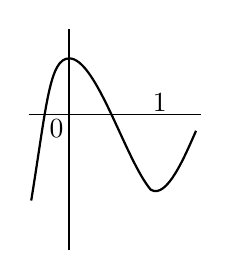
\begin{tikzpicture}[line width=0.6pt,scale=1.15]
  \draw (-0.45,0) -- (1.45,0);
  \draw (0,-1.5) -- (0,0.95);
  \node at (-0.14,-0.16) {$0$};
  \node at (1.0,0.13) {$1$};
  \draw[line width=0.8pt] (-0.42,-0.95)
    .. controls (-0.25,0.1) and (-0.22,0.62) .. (0,0.62)
    .. controls (0.3,0.62) and (0.62,-0.5) .. (0.9,-0.83)
    .. controls (1.08,-0.94) and (1.28,-0.45) .. (1.4,-0.18);
\end{tikzpicture}
\caption{函数 $g$}
\label{fig:function-g}
\end{figure}

函数 $\widetilde{F}=F+g\colon V\times\bigl[-\tfrac{1}{3},\tfrac{4}{3}\bigr]\to\RR$ 是一个\trMorseFunction，其\trCriticalPoint{}为
\[
\operatorname{Crit}\bigl(\widetilde{F}\bigr)
  =\operatorname{Crit}(f_0)\times\{0\}\cup\operatorname{Crit}(f_1)\times\{1\}\text{。}
\]
此外，对 $a\in\operatorname{Crit}(f_0)$，
\[
\operatorname{Ind}_{\widetilde{F}}(a,0)=\operatorname{Ind}_{f_0}(a)+1\text{，}
\]
而对 $b\in\operatorname{Crit}(f_1)$，\footnote{译注：原书此式印作 $\operatorname{Ind}_{f_0}(b)$；因在 $s=1$ 附近 $\widetilde{F}=f_1+g$，而 $g$ 的\trCriticalPoint{} $1$ 是极小值点（\trIndex{}为 $0$），故应为 $\operatorname{Ind}_{f_1}(b)$；此处径改。——译者注}则有
\[
\operatorname{Ind}_{\widetilde{F}}(b,1)=\operatorname{Ind}_{f_1}(b)\text{。}
\]

利用一个\trPartitionOfUnity，我们构造一个\trAdapted{}于 $\widetilde{F}$ 的\trPseudogradient{}场 $X$，它在
\[
\begin{cases}
X_0-\operatorname{grad}g & \text{在 } V\times\bigl[-\tfrac{1}{3},\tfrac{1}{3}\bigr]\text{ 上}\\
X_1-\operatorname{grad}g & \text{在 } V\times\bigl[\tfrac{2}{3},\tfrac{4}{3}\bigr]\text{ 上}
\end{cases}
\]
与之相重合（当然，其中 $\operatorname{grad}g$ 表示 $g$ 的\trEuclidean{}\trGradient）。这样，$X$ 便与 $V\times\bigl[-\tfrac{1}{3},\tfrac{4}{3}\bigr]$ 的边界\trTransverse。我们用一个具有\trSmaleCondition{}的小\trPerturbation{} $\widetilde{X}$ 来替换 $X$，并且我们可以——而且我们也确实——假定：它与诸\trSection{} $V\times\{s\}$（$s\in\{-1/3,\,1/3,\,2/3,\,4/3\}$）\trTransverse。请注意，一个满足\trSmaleCondition{}的\trAdapted{}\trPseudogradient{}场的小\trPerturbation{}，是一个具有同样性质的\trAdapted{}\trPseudogradient{}场……并且连接两个\trIndex{}相邻的\trCriticalPoint{}的诸\trTrajectory{}的数目也相同（两个场的诸\trTrajectory{}所成之集之间存在一个\trBijective）。这就是下面这条命题所表述的内容。

\begin{proposition}\label{thm:perturbation-smale}
设 $f\colon V\to\RR$ 是一个\trMorseFunction，并设 $X$ 是一个\trAdapted{}于 $f$ 的、具有\trSmaleCondition{}的\trPseudogradient{}场。充分贴近 $X$（在 $\cC^1$ 意义下）的每个\trVectorField{} $\widetilde{X}$，都是一个仍具有\trSmaleCondition{}的\trAdapted{}\trPseudogradient{}场。\footnote{译注：此断言按字面不真：任意的 $\cC^1$ 小\trPerturbation{}未必仍是\trAdapted{}的。局部反例：取 $f=x^2$、$X=-2x\,\partial_x$，以紧支截断取 $\widetilde{X}=X+\varepsilon\,\partial_x$（任意小），则在 $0<x<\varepsilon/2$ 处 $df(\widetilde{X})=2x\,(-2x+\varepsilon)>0$，$\widetilde{X}$ 不再\trAdapted{}于 $f$。故\trPerturbation{}须限于 $f$ 的\trAdapted{}\trPseudogradient{}所成之空间内（或在固定诸临界邻域之外进行）。此处照原书排印，存疑备案。——译者注}此外，我们有
\[
\bigl(C_{\star}(f),\partial_X\bigr)=\bigl(C_{\star}(f),\partial_{\widetilde{X}}\bigr)
\]
\noqed
\end{proposition}

因此，我们可以选取 $\widetilde{X}$，\footnote{译注：原书自首构造 $X_i-\operatorname{grad}g$ 之后的诸\trInterpolation{}与边界公式中均印作 $+\operatorname{grad}g$；按\trAdapted{}条件与\trTrajectory{}方向推演，疑均应作 $-\operatorname{grad}g$；本节一并径改。又，下式末项原书印作 $C_{\star+1}(f_0)$，由 $\operatorname{Ind}_{\widetilde{F}}(a,0)=\operatorname{Ind}_{f_0}(a)+1$ 应为 $C_{\star-1}(f_0)$（与下文 $C_{k+1}(\widetilde{F})=C_k(f_0)\oplus C_{k+1}(f_1)$ 相合）；亦径改。——译者注}使得\footnote{译注：原书中间一项印作 $g\bigl|_{[-1/3,\,2/3]}$；据左端 $\widetilde{F}$ 的限制区间，应为 $g\bigl|_{[-1/3,\,1/3]}$；此处径改。——译者注}
\[
\begin{aligned}
\bigl(C_{\star}\bigl(\widetilde{F}\bigr|_{V\times[-\frac{1}{3},\frac{1}{3}]}\bigr),\partial_{\widetilde{X}}\bigr)
  &=\bigl(C_{\star}\bigl(f_0+g\bigr|_{[-\frac{1}{3},\frac{1}{3}]}\bigr),\partial_{X_0-\operatorname{grad}g}\bigr)\\
  &=\bigl(C_{\star-1}(f_0),\partial_{X_0}\bigr)
\end{aligned}
\]
并且类似地，使得
\[
\begin{aligned}
\bigl(C_{\star}\bigl(\widetilde{F}\bigr|_{V\times[\frac{2}{3},\frac{4}{3}]}\bigr),\partial_{\widetilde{X}}\bigr)
  &=\bigl(C_{\star}\bigl(f_1+g\bigr|_{[\frac{2}{3},\frac{4}{3}]}\bigr),\partial_{X_1-\operatorname{grad}g}\bigr)\\
  &=\bigl(C_{\star}(f_1),\partial_{X_1}\bigr)\text{。}
\end{aligned}
\]

现在让我们来考虑与\trMorseFunction{} $\widetilde{F}$ 及场 $\widetilde{X}$ 相伴的、乘积 $V\times\bigl[-\tfrac{1}{3},\tfrac{4}{3}\bigr]$ 上的那个\trComplex。$\widetilde{X}$ 的连接 $\widetilde{F}$ 的两个\trCriticalPoint{}的诸\trTrajectory{}可以分成两类：留在\trSection{} $s\in\bigl[-\tfrac{1}{3},\tfrac{1}{3}\bigr]$ 或\trSection{} $s\in\bigl[\tfrac{2}{3},\tfrac{4}{3}\bigr]$ 中的那些——它们是 $X_0$ 或 $X_1$ 的\trTrajectory——以及从一个 $f_0$ 的\trCriticalPoint{}（在\trSection{} $s\in\bigl[-\tfrac{1}{3},\tfrac{1}{3}\bigr]$ 中）走到一个 $f_1$ 的\trCriticalPoint{}（在\trSection{} $s\in\bigl[\tfrac{2}{3},\tfrac{4}{3}\bigr]$ 中）的那些。我们有
\[
C_{k+1}\bigl(\widetilde{F}\bigr)=C_k(f_0)\oplus C_{k+1}(f_1)\text{。}
\]

考虑到上述内容，在此分解中，
\[
\partial_{\widetilde{X}}\colon C_k(f_0)\oplus C_{k+1}(f_1)
  \longrightarrow C_{k-1}(f_0)\oplus C_k(f_1)
\]
具有如下形式的矩阵：
\[
\partial_{\widetilde{X}}
  =\begin{pmatrix}\partial_{X_0} & 0\\ \Phi^F & \partial_{X_1}\end{pmatrix}\text{。}
\]
元素
\[
\Phi^F\colon C_k(f_0)\longrightarrow C_k(f_1)
\]
由
\[
\Phi^F(a)=\sum_{b\in\operatorname{Crit}_k(f_1)} n_{\widetilde{X}}(a,b)\,b
\]
给出，其中 $n_{\widetilde{X}}(a,b)$ 清点着 $\widetilde{X}$ 的那些连接 $a\in V\times\{0\}\cap\operatorname{Crit}\bigl(\widetilde{F}\bigr)$ 与 $b\in V\times\{1\}\cap\operatorname{Crit}\bigl(\widetilde{F}\bigr)$ 的\trTrajectory。关系式 $\partial_{\widetilde{X}}\circ\partial_{\widetilde{X}}=0$ 给出
\[
\Phi^F\circ\partial_{X_0}+\partial_{X_1}\circ\Phi^F=0
\qquad\text{亦即}\qquad
\Phi^F\circ\partial_{X_0}=\partial_{X_1}\circ\Phi^F\text{，}
\]
从而 $\Phi^F$ 确实是\trComplex{}的一个\trMorphism。

\emph{第二步。}

如果 $f_1=f_0$ 且 $X_0=X_1$，那么我们从
\[
I\colon V\times[0,1]\longrightarrow\RR\text{，}\qquad
I(x,s)=f_0(x)\ \text{（对每个 } s\text{）}
\]
出发，并且像上面那样使用一个函数 $g$。\trVectorField{} $X=X_0-\operatorname{grad}g$ 是一个\trAdapted{}\trPseudogradient{}场，并且满足\trSmaleCondition。此外，对 $f_0$ 的每个\trCriticalPoint{} $a$，都存在 $X$ 的一条唯一的\trTrajectory，它连接 $(a,0)$ 与 $(c,1)$，其中 $\operatorname{Ind}_{f_0}(a)=\operatorname{Ind}_{f_0}(c)$：这就是连接 $(a,0)$ 与 $(a,1)$ 的那条在 $V$ 上的投影为常值的\trTrajectory。于是，$\Phi^I=\operatorname{Id}$。

\emph{第三步。}

现在，我们有了分别从 $f_0$ 到 $f_1$、从 $f_1$ 到 $f_2$ 与从 $f_0$ 到 $f_2$ 的\trInterpolation{} $F$、$G$ 与 $H$。我们通过选取一个函数\footnote{译注：原书下式第二个区间印作 $\bigl[\tfrac{1}{3},\tfrac{4}{3}\bigr]$；据下文 $t\in[-\tfrac{1}{3},\tfrac{1}{3}]$ 时 $K_{s,t}=F_s$ 之要求，$t$ 须可取到 $-\tfrac{1}{3}$，应为 $\bigl[-\tfrac{1}{3},\tfrac{4}{3}\bigr]$；此处径改。——译者注}
\[
K\colon V\times\bigl[-\tfrac{1}{3},\tfrac{4}{3}\bigr]\times\bigl[-\tfrac{1}{3},\tfrac{4}{3}\bigr]\longrightarrow\RR\text{，}\qquad
K(x,s,t)=K_{s,t}(x)
\]
来在这些函数之间进行\trInterpolation，它满足\cref{fig:k-diagram}所概括的那些性质：

\begin{figure}[htbp]
\centering
\begin{tikzpicture}[line width=0.6pt,scale=3.2]
  \fill[gray!55] (-1/3,2/3) rectangle (4/3,4/3);
  \fill[gray!55] (-1/3,-1/3) rectangle (1/3,1/3);
  \fill[gray!55] (2/3,-1/3) rectangle (4/3,1/3);
  \draw[line width=1.1pt] (-1/3,-1/3) rectangle (4/3,4/3);
  \draw[line width=1.1pt] (-1/3,1) -- (4/3,1);
  \draw[line width=1.1pt] (1,-1/3) -- (1,4/3);
  \draw[->] (-0.55,0) -- (1.72,0) node[below right] {$s$};
  \draw[->] (0,-0.62) -- (0,1.52) node[right] {$t$};
  \node at (-0.46,-0.17) {$-\tfrac{1}{3}$};
  \node at (1.45,-0.17) {$\tfrac{4}{3}$};
  \node at (-0.17,1.44) {$\tfrac{4}{3}$};
  \node at (-0.17,-0.56) {$-\tfrac{1}{3}$};
  \node at (0.13,-0.49) {$H$};
  \node at (1.02,-0.49) {$G$};
  \node at (1.46,0.11) {$F$};
  \node at (0.1,0.14) {$f_0$};
  \node at (1.1,0.14) {$f_1$};
  \node at (1.5,1.0) {$f_2$};
\end{tikzpicture}
\caption{}
\label{fig:k-diagram}
\end{figure}

\begin{itemize}
\item 对 $s\in[-1/3,\,1/3]$，$K_{s,t}=H_t$。
\item 对 $s\in[2/3,\,4/3]$，$K_{s,t}=G_t$。
\item 对 $t\in[-1/3,\,1/3]$，$K_{s,t}=F_s$。
\item 对 $t\in[2/3,\,4/3]$，$K_{s,t}=f_2$。
\end{itemize}

我们还要使用一个像前面所用那样的\trMorseFunction{} $g\colon\RR\to\RR$（其图象见于\cref{fig:function-g}），它仅有的\trCriticalPoint{}是\trIndex{}为 $1$ 的 $0$ 与\trIndex{}为 $0$ 的 $1$，在 $[0,1]$ 之外递增，并且满足
\[
\frac{\partial K}{\partial s}(x,s,t)+g'(s)<0
\qquad\text{对所有的 } (x,s,t)\in V\times\,]0,1[\,\times\bigl[\tfrac{1}{3},\tfrac{4}{3}\bigr]
\]
以及
\[
\frac{\partial K}{\partial t}(x,s,t)+g'(t)<0
\qquad\text{对所有的 } (x,s,t)\in V\times\bigl[\tfrac{1}{3},\tfrac{4}{3}\bigr]\times\,]0,1[\text{。}
\]
最后，令 $\widetilde{K}$ 是由
\[
\widetilde{K}(x,s,t)=K_{s,t}(x)+g(s)+g(t)
\]
定义的函数。

由于 $g$ 的这一取法，$\widetilde{K}$ 的诸\trCriticalPoint{}都位于\cref{fig:k-diagram}的阴影区域之中，在那里 $\widetilde{K}(x,s,t)$ 可以写成 $f_i(x)+g(s)+g(t)$（$i=0$、$1$ 或 $2$）。特别地，它是一个\trMorseFunction，其\trCriticalPoint{}为
\[
\begin{aligned}
\operatorname{Crit}\bigl(\widetilde{K}\bigr)
  =\bigl[\operatorname{Crit}(f_0)\times\{0\}\times\{0\}\bigr]
   \cup\bigl[\operatorname{Crit}(f_1)\times\{1\}\times\{0\}\bigr]\\
  \cup\bigl[\operatorname{Crit}(f_2)\times\{0\}\times\{1\}\bigr]
   \cup\bigl[\operatorname{Crit}(f_2)\times\{1\}\times\{1\}\bigr]\text{。}
\end{aligned}
\]
这些\trCriticalPoint{}的\trIndex{}如下：
\begin{itemize}
\item 若 $a\in\operatorname{Crit}(f_0)$，则 $\operatorname{Ind}_{\widetilde{K}}(a,0,0)=\operatorname{Ind}_{f_0}(a)+2$。
\item 若 $b\in\operatorname{Crit}(f_1)$，则 $\operatorname{Ind}_{\widetilde{K}}(b,1,0)=\operatorname{Ind}_{f_1}(b)+1$。
\item 若 $c\in\operatorname{Crit}(f_2)$，则
\[
\operatorname{Ind}_{\widetilde{K}}(c,0,1)=\operatorname{Ind}_{f_2}(c)+1
\qquad\text{并且}\qquad
\operatorname{Ind}_{\widetilde{K}}(c,1,1)=\operatorname{Ind}_{f_2}(c)\text{。}
\]
\end{itemize}

设 $X$ 表示上面构造的、\trAdapted{}于 $\widetilde{F}$ 的那个\trPseudogradient{}场，而 $Y$ 表示\trAdapted{}于 $\widetilde{G}=G+g$ 的那一个。再一次利用一个\trPartitionOfUnity，我们定义一个\trAdapted{}于 $\widetilde{K}$ 的\trPseudogradient{}场 $\mathcal{X}$，使得：
\begin{itemize}
\item 对 $s\in[-1/3,\,1/3]$，$\mathcal{X}(x,s,t)=Z(x,t)-\operatorname{grad}g(s)$，其中 $Z$ 是
\[
H(x,t)+g(t)\colon V\times\bigl[-\tfrac{1}{3},\tfrac{4}{3}\bigr]\longrightarrow\RR
\]
的一个\trPseudogradient。
\item 对 $s\in[2/3,\,4/3]$，$\mathcal{X}(x,s,t)=Y(x,t)-\operatorname{grad}g(s)$，其中 $Y$ 是 $\widetilde{G}$ 的一个\trPseudogradient。
\item 对 $t\in[-1/3,\,1/3]$，$\mathcal{X}(x,s,t)=X(x,s)-\operatorname{grad}g(t)$。
\item 对 $t\in[2/3,\,4/3]$，$\mathcal{X}(x,s,t)=X_2-\operatorname{grad}g(s)-\operatorname{grad}g(t)$。
\end{itemize}

然后，我们取 $\mathcal{X}$ 的一个\trPerturbation{} $\widetilde{\mathcal{X}}$，以便使之满足\trSmaleCondition，并且（如同在第一步中那样）假定：在 $V\times\,]1/3,2/3[\,\times\,]1/3,2/3[$ 之外，$\widetilde{\mathcal{X}}$ 的连接\trIndex{}相邻的\trCriticalPoint{}的诸\trTrajectory{}与 $\mathcal{X}$ 的那些\trTrajectory{}一一对应（\cref{thm:perturbation-smale}）。

现在让我们来考虑与 $\widetilde{K}$ 及 $\widetilde{\mathcal{X}}$ 相伴的\trCriticalPoint{}\trComplex。\trManifold{} $V\times[-1/3,\,4/3]\times[-1/3,\,4/3]$\footnote{译注：原书印刷~74 处第一个区间印作 $\bigl[-\tfrac{1}{2},\tfrac{4}{3}\bigr]$；全节他处皆为 $-\tfrac{1}{3}$（见上文 $\widetilde{F}$ 的定义域），疑系排印笔误；此处径改。又，印刷~72 处 $K$ 的定义域第二个区间印作 $\bigl[\tfrac{1}{3},\tfrac{4}{3}\bigr]$，疑漏一枚负号，系独立疑误，已于前文该式处另注径改。——译者注}并不具有一个（\trSmooth{}的）边界，但\cref{thm:cornered-boundary}的条件却得到满足。我们有
\[
C_{k+1}\bigl(\widetilde{K}\bigr)
  =C_{k-1}(f_0)\oplus C_k(f_1)\oplus C_k(f_2)\oplus C_{k+1}(f_2)\text{。}
\]

\cref{fig:diagram-morphisms}中的图表展示了我们所使用的各个\trMorphism{}之间的联系。在此分解中，\trDifferential{}可以写成
\[
\partial_{\widetilde{\mathcal{X}}}=
\begin{pmatrix}
\partial_{X_0} & 0 & 0 & 0\\
\Phi^F & \partial_{X_1} & 0 & 0\\
\Phi^H & 0 & \partial_{X_2} & 0\\
S & \Phi^G & \operatorname{Id} & \partial_{X_2}
\end{pmatrix}\text{。}
\]
恒等式 $\partial_{\widetilde{\mathcal{X}}}\circ\partial_{\widetilde{\mathcal{X}}}=0$ 给出
\[
S\circ\partial_{X_0}+\Phi^G\circ\Phi^F+\Phi^H+\partial_{X_2}\circ S=0
\]
亦即\footnote{译注：原书上行末式印作 $S\circ\partial_{X_0}+\Phi^G\circ\Phi^F+\Phi^H+\partial_{X_2}\circ S=0$，在 $\ZZ$ 系数下与下式 $\Phi^G\circ\Phi^F-\Phi^H=S\circ\partial_{X_0}+\partial_{X_2}\circ S$ 不\trCompatible。本段矩阵计算须先在 $\ZZ/2$ 系数下理解；若扩展到 $\ZZ$ 系数，须对移位\trComplex{}统一调整\trOrientation{}与\trHomotopy{}符号，非单一改一处符号所能解决；此处照原书排印，存疑备案。——译者注}
\[
\Phi^G\circ\Phi^F-\Phi^H=S\circ\partial_{X_0}+\partial_{X_2}\circ S\text{。}
\]

\begin{figure}[htbp]
\centering
\begin{tikzpicture}[line width=0.7pt,scale=1.0]
  \newcommand{\planebody}{%
    \draw (0,0) -- (1.5,0.8) -- (1.5,3.4) -- (0,2.6) -- cycle;
    \fill (0.79,2.41) circle (1.3pt);
    \draw (0.79,2.41) .. controls (0.95,2.15) .. (0.97,1.95);
    \draw[->] (0.97,1.95) .. controls (0.99,1.65) and (0.95,1.35) .. (0.79,1.13);
    \fill (0.79,1.13) circle (1.3pt);}
  \newcommand{\planebottom}[1]{\node[inner sep=1.5pt] at (1.45,0.12) {#1};}
  \begin{scope}[shift={(0,0)}]
    \planebody
    \node at (0.87,2.64) {$a$};
    \node at (1.32,1.55) {$\partial_{X_0}$};
    \planebottom{$V\times 0\times 0$}
  \end{scope}
  \begin{scope}[shift={(4.1,0)}]
    \planebody
    \node at (1.32,1.55) {$\partial_{X_1}$};
    \planebottom{$V\times 1\times 0$}
  \end{scope}
  \begin{scope}[shift={(0,-3.94)}]
    \planebody
    \node at (1.32,1.55) {$\partial_{X_2}$};
    \planebottom{$V\times 0\times 1$}
  \end{scope}
  \begin{scope}[shift={(4.1,-3.94)}]
    \planebody
    \node at (1.32,1.55) {$\partial_{X_2}$};
    \planebottom{$V\times 1\times 1$}
  \end{scope}
  \draw[->] (2.24,1.70) -- (3.76,1.70) node[midway,above] {$\Phi^F$};
  \draw[->] (0.76,-0.05) -- (0.76,-0.82) node[midway,right] {$\Phi^H$};
  \draw[->] (4.86,-0.05) -- (4.86,-0.82) node[midway,right] {$\Phi^G$};
  \draw[->] (2.2,-2.38) -- (3.76,-2.38) node[midway,above] {$\operatorname{Id}$};
  \draw[->] (1.84,0.73) -- (3.71,-1.47) node[pos=0.6,above=3mm] {$S$};
\end{tikzpicture}
\caption{}
\label{fig:diagram-morphisms}
\end{figure}

由此我们推出：$\Phi^G\circ\Phi^F$ 与 $\Phi^H$ 在\trHomology{}中诱导出相同的\trMorphism。
\end{proof}
